\appendix

\section{Structures, sizes and representation}
\label{sec:representation}

\Cref{fig:molecules} shows six dataset molecules and \cref{fig:distributions} the atom- and bond-count distributions summarised in \cref{tab:audit}.

\begin{figure}[tb]
    \centering
    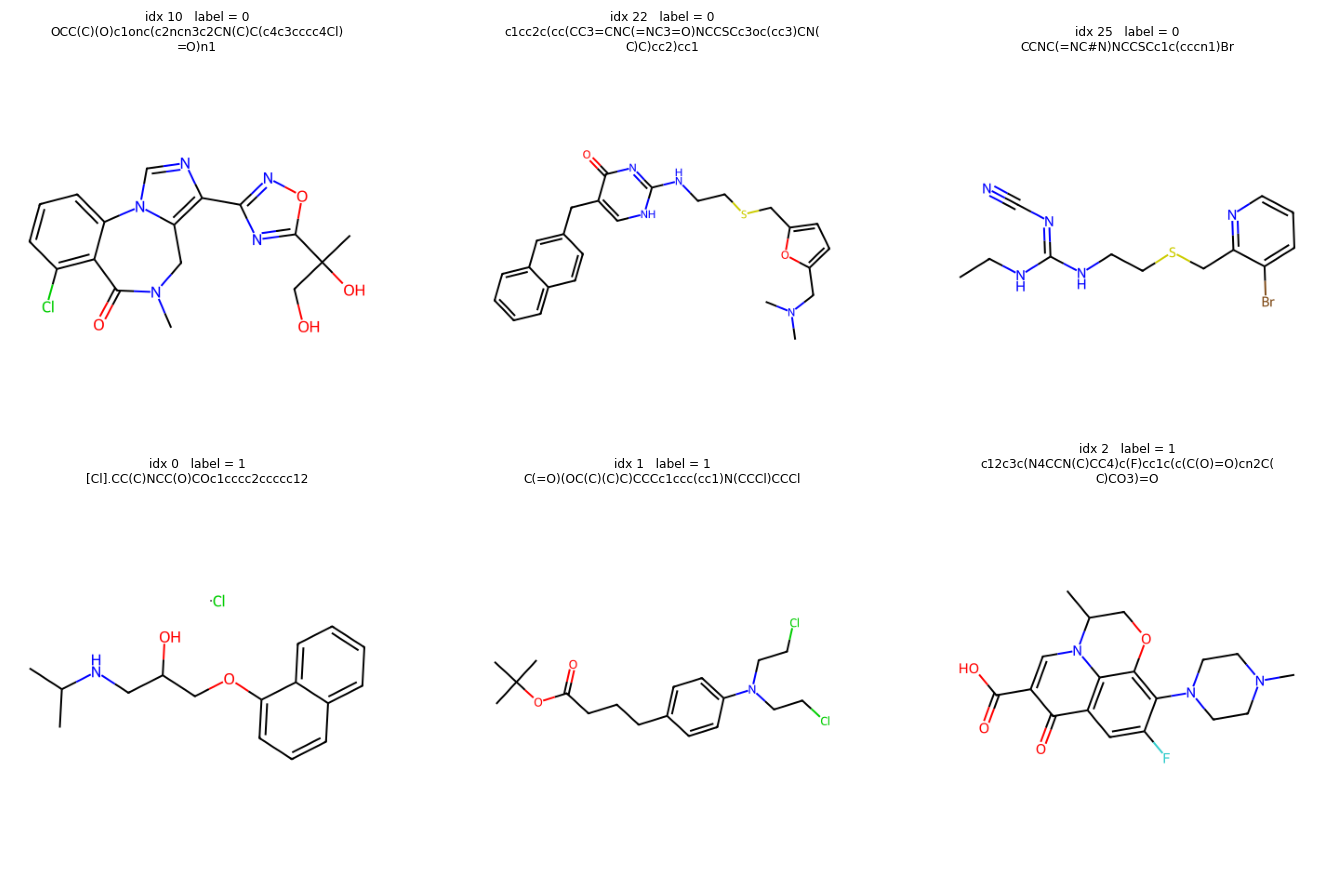
\includegraphics[width=\columnwidth]{Images/molecules.png}
    \caption{%
        Six dataset molecules with their SMILES strings: three non-penetrating (label 0, top) and three penetrating (label 1, bottom). Hydrogens are implicit; dataset index and label are given above each structure.
     }%
   \label{fig:molecules}
\end{figure}

\begin{figure}[tb]
    \centering
    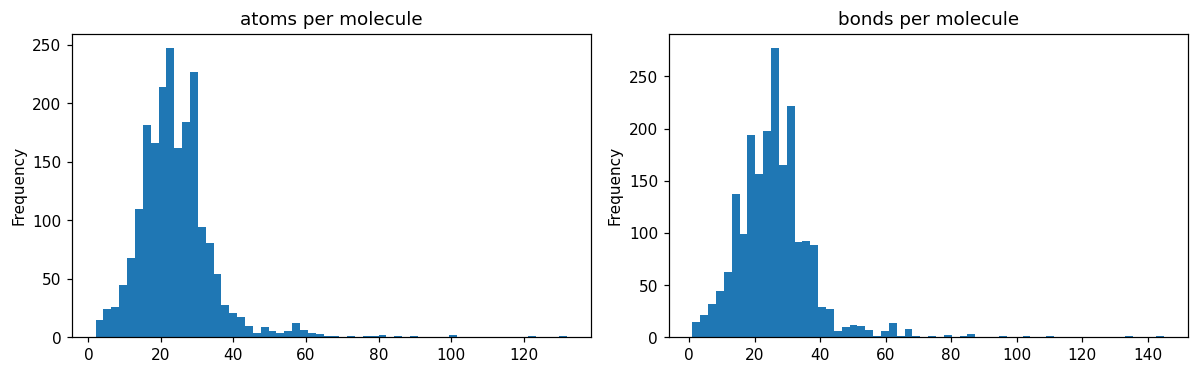
\includegraphics[width=\columnwidth]{Images/distributions.png}
    \caption{%
        Atom count (left) and bond count (right) over the 2039 loaded molecules; bonds are counted once, not once per direction.
     }%
   \label{fig:distributions}
\end{figure}

\begin{figure}[tb]
    \centering
    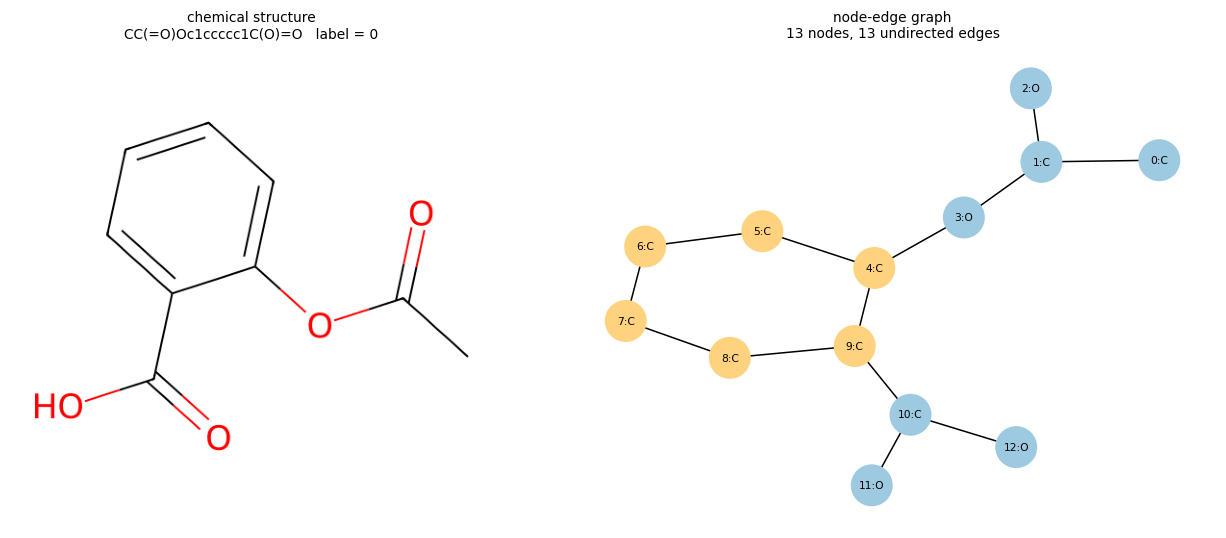
\includegraphics[width=\columnwidth]{Images/graph-view.png}
    \caption{%
        Acetylsalicylic acid (index 98) as a chemical depiction and as the graph the model consumes. Node $i$ on the right is atom $i$ on the left; orange nodes are the six aromatic ring atoms, blue the acetyl and carboxyl substituents.
     }%
   \label{fig:graph-view}
\end{figure}

The first graph of the dataset has \texttt{x.shape} $= (20, 9)$, \texttt{edge\_index.shape} $= (2, 40)$, \texttt{edge\_attr.shape} $= (40, 3)$ and label $y = 1$ --- propranolol hydrochloride, whose 40 edge entries are 20 bonds stored in both directions. Decoding confirms that the attributes are indices rather than values: formal-charge code 5 is charge 0 and code 7 is charge $+2$, hybridisation code 3 is SP2 and code 4 is SP3. Encoding by \cref{eq:atom-encoder} with $d=64$ maps $x$ to $(20,64)$ and \texttt{edge\_attr} to $(40,64)$. \Cref{fig:graph-view} places the chemical depiction beside the graph, and the two agree exactly: 13 atoms as 13 nodes, 13 bonds as 13 undirected edges, with RDKit's atomic numbers equal to the first attribute column. Batching 32 molecules yields \texttt{x} $(778,9)$, \texttt{edge\_index} $(2,1664)$, \texttt{edge\_attr} $(1664,3)$, a graph-assignment vector of length 778 with values $0 \ldots 31$ and $y$ of shape $(32,1)$ --- one label per graph, not per atom --- with graph 1 starting at atom 20, exactly the atom count of graph 0.

\section{Per-run training outcome}

\begin{table}[htb]
    \centering
    \caption{Per-run training outcome. Validation ROC-AUC is the value at the restored checkpoint; ``best ep.'' is the epoch of that checkpoint.}
    \label{tab:seeds}
    \footnotesize
    \begin{tabular}{@{}llrrr@{}}
        \toprule
        Split & Seed & Val.\ AUC & Best ep. & Epochs \\
        \midrule
        Random   & 0 & 0.9130 & 28 &  54 \\
                 & 1 & 0.9171 & 30 &  56 \\
                 & 2 & 0.9162 & 74 & 100 \\
        \midrule
        Scaffold & 0 & 0.8804 & 54 &  80 \\
                 & 1 & 0.8822 & 69 &  95 \\
                 & 2 & 0.8773 & 44 &  70 \\
        \bottomrule
    \end{tabular}
\end{table}

\section{Attribute vocabularies}
\label{sec:vocab}

Reserved but unused slots are the reason an embedding table is preferable to one-hot encoding for \texttt{atomic\_\allowbreak{}num}, where 119 slots exist and 13 occur.

\begin{table}[htb]
    \centering
    \caption{Categorical attribute columns, vocabulary sizes and observed values.}
    \label{tab:featuremaps}
    \scriptsize
    \setlength{\tabcolsep}{4pt}
        \begin{tabular}{@{}rp{0.27\columnwidth}rp{0.30\columnwidth}@{}}
        \toprule
        Col & Attribute & Slots & Observed \\
        \midrule
        \multicolumn{4}{@{}l}{\textit{Atom attributes,} $x$ \textit{, shape} $(49\,068, 9)$} \\
        0 & \texttt{atomic\_\allowbreak{}num}            & 119 & 13 elements: H, B, C, N, O, F, Na, \ldots \\
        1 & \texttt{chirality}             &   9 & 3: unspecified, tetrahedral CW, tetrahedral CCW \\
        2 & \texttt{degree}                &  11 & 5: 0--4 \\
        3 & \texttt{formal\_\allowbreak{}charge}         &  12 & 4: $-1$, 0, $+1$, $+2$ \\
        4 & \texttt{num\_hs}                &   9 & 4: 0--3 \\
        5 & \texttt{num\_radical\_\allowbreak{}electrons} &   5 & 2: 0, 1 \\
        6 & \texttt{hybridi\allowbreak{}zation}         &   8 & 4: S, SP, SP2, SP3 \\
        7 & \texttt{is\_aromatic}           &   2 & 2: false, true \\
        8 & \texttt{is\_in\_ring}            &   2 & 2: false, true \\
        \midrule
        \multicolumn{4}{@{}l}{\textit{Bond attributes,} \texttt{edge\_attr} \textit{, shape} $(105\,842, 3)$} \\
        0 & \texttt{bond\_type}             &  22 & 4: single, double, triple, aromatic \\
        1 & \texttt{stereo}                &   6 & 3: none, Z, E \\
        2 & \texttt{is\_\allowbreak{}conjugated}         &   2 & 2: false, true \\
        \bottomrule
    \end{tabular}
\end{table}

\section{Molecules with contradictory labels}

The ten canonical SMILES in \cref{tab:conflicts} occur twice in the file with both labels and were removed before splitting. They are ordinary, well-characterised drugs, which is why the contradiction is attributable to the dataset's assembly rather than to exotic chemistry.

\begin{table}[htb]
    \centering
    \caption{The ten canonical SMILES carrying both labels (20 records removed).}
    \label{tab:conflicts}
    \scriptsize
    \setlength{\tabcolsep}{4pt}
    \begin{tabular}{@{}p{0.60\columnwidth}l@{}}
        \toprule
        Canonical SMILES & Common name \\
        \midrule
        \smiles{CC(=O)Oc1ccccc1C(=O)O} & acetylsalicylic acid \\
        \smiles{N[C@@H](Cc1ccc(O)c(O)c1)C(=O)O} & levodopa \\
        \smiles{CN1C2CCC1CC(OC(=O)C(CO)c1ccccc1)C2} & atropine \\
        \smiles{CCOC(=O)N1CCC(=C2c3ccc(Cl)cc3CCc3cccnc32)CC1} & loratadine \\
        \smiles{CN(C)C(=O)C(CCN1CCC(O)(c2ccc(Cl)cc2)CC1)(c1ccccc1)c1ccccc1} & loperamide \\
        \smiles{COc1cc(NCc2ccc3nc(N)nc(N)c3c2C)cc(OC)c1OC} & trimetrexate \\
        \smiles{COc1ccc2c(c1)c(CC(=O)O)c(C)n2C(=O)c1ccc(Cl)cc1} & indometacin \\
        \smiles{C[C@H]1C[C@@H]2[C@H]([C@@H](O)C[C@@]3(C)[C@H]2CC[C@]3(O)C(=O)CO)[C@@]2(C)C=CC(=O)C=C12} & a corticosteroid \\
        \smiles{Clc1ccc(COC(Cn2ccnc2)c2ccc(Cl)cc2Cl)c(Cl)c1} & an azole antifungal \\
        \smiles{c1ccc2c(c1)Sc1ccccc1N2CC1CN2CCC1CC2} & a phenothiazine \\
        \bottomrule
    \end{tabular}
\end{table}

\section{Most confident errors}

\begin{figure}[tb]
    \centering
    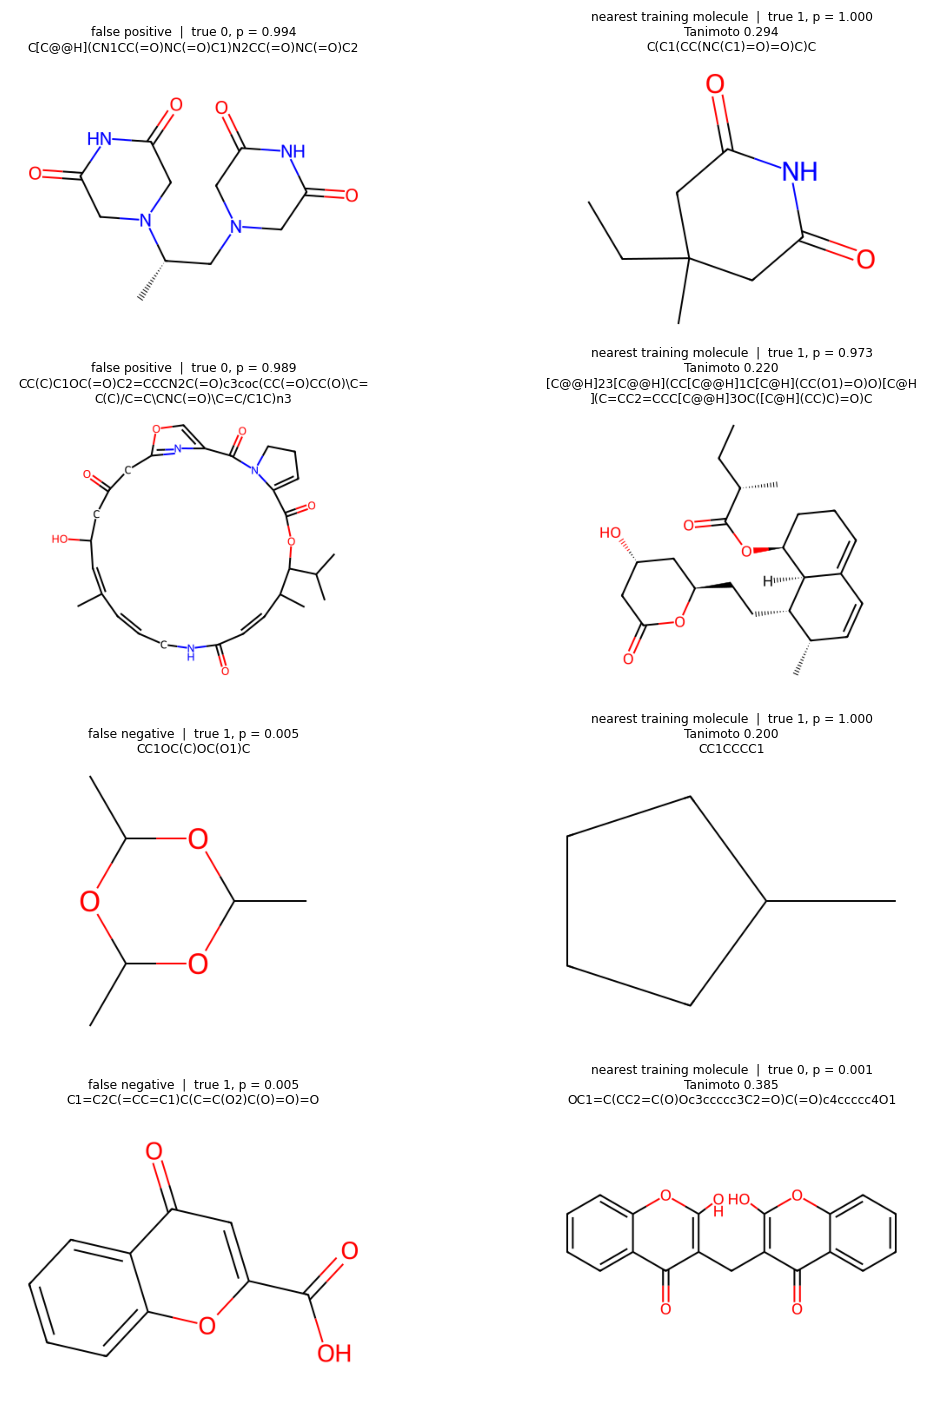
\includegraphics[width=0.84\columnwidth]{Images/errors.png}
    \caption{%
        The four most confident test errors of the scaffold-split network (seed 2, threshold 0.832) beside their nearest training molecule by Tanimoto similarity on ECFP4. Rows 1--2 are the false positives, rows 3--4 the false negatives; each title gives the true label and the predicted probability.
     }%
   \label{fig:errors}
\end{figure}

\begin{table}[htb]
    \centering
    \caption{The four most confident test errors of the scaffold-split network (seed 2, frozen threshold 0.832) and their nearest training molecule. FP and FN are false positive and false negative, $p$ the predicted probability, $T$ the Tanimoto similarity on ECFP4 to the nearest training molecule and $\bar{T}$ the mean over the whole training subset; the last column (Nb.) gives that neighbour's true label and predicted probability. The median nearest-neighbour similarity over the scaffold test subset is 0.400.}
    \label{tab:errors}
    \scriptsize
    \setlength{\tabcolsep}{2.5pt}
    \begin{tabular}{@{}llccccc@{}}
        \toprule
        Molecule & Type & True & $p$ & $T$ & $\bar{T}$ & Nb. \\
        \midrule
        Bis-glutarimide      & FP & 0 & 0.994 & 0.294 & 0.096 & 1, 0.999 \\
        Macrocyclic polyket. & FP & 0 & 0.989 & 0.220 & 0.088 & 1, 0.973 \\
        Cyclic acetal        & FN & 1 & 0.005 & 0.200 & 0.033 & 1, 1.000 \\
        Chromone-2-c.\ acid  & FN & 1 & 0.005 & 0.385 & 0.115 & 0, 0.001 \\
        \bottomrule
    \end{tabular}
\end{table}

\section{Integrity and reproducibility}
\label{sec:integrity}
\label{sec:repro}

Iterating the whole dataset through the loader in batches of 64 reproduced 2039 graphs and \num{49068} atoms, with all labels finite, every graph holding at least one atom, and the number of labels equal to the number of graphs in every batch. Both splits covered all 1965 molecules with pairwise disjoint indices and zero shared canonical SMILES.

Every number in this report comes from one top-to-bottom execution of the accompanying notebook, which takes about \SI{2.5}{\minute} on CPU. The split seed is 42 and controls stratification, scaffold tie-breaking and the baseline solver; the network seeds are 0, 1 and 2 and control initialisation, dropout masks and batch order. Training is deterministic on CPU at these seeds, so a re-run reproduces the reported values exactly. The repository linked on the title page holds the executed notebook with all outputs, a \texttt{README.md} giving the run order and a \texttt{requirements.txt} pinning the environment.
\appendixfootnote{The notebook holds the code; this report holds the interpretation.}
